\documentclass[conference]{IEEEtran}
\IEEEoverridecommandlockouts
% The preceding line is only needed to identify funding in the first footnote. If that is unneeded, please comment it out.
\usepackage{cite}
\usepackage{amsmath,amssymb,amsfonts}
\usepackage{algorithmic}
\usepackage{graphicx}
\usepackage{textcomp}
\usepackage{xcolor}
\usepackage{multirow}
\usepackage{float}
\def\BibTeX{{\rm B\kern-.05em{\sc i\kern-.025em b}\kern-.08em
    T\kern-.1667em\lower.7ex\hbox{E}\kern-.125emX}}
\begin{document}

\title{An Initial Study About the Impact of Handwriting and Keyboard Keystroke Dynamics Combination to Emotional State Prediction\\
% {\footnotesize \textsuperscript{*}Note: Sub-titles are not captured in Xplore and
% should not be used}
% \thanks{This work has been financially supported by CNPq/Brazil, under process numbers 1762337.}
}

% \author{\IEEEauthorblockN{Danilo R. C. Bandeira and Anne M. P. Canuto}
% \IEEEauthorblockA{\textit{Dept. of Informatics and Applied Mathematics - DIMAp} \\
% \textit{Federal University of Rio Grande do Norte - UFRN}\\
% Natal, Brazil \\
% danilorodrigo@ppgsc.ufrn.br, anne@dimap.ufrn.br}
% \and
% \IEEEauthorblockN{Michael Fairhurst and Cheng Li}
% \IEEEauthorblockA{\textit{School of Engineering and Digital Arts} \\
% \textit{University of Kent}\\
% Canterbury, England \\
% m.fairhurst@kent.ac.uk, durrrivey@outlook.com}
% % \and
% % \IEEEauthorblockN{Diego S. C. Nascimento}
% % \IEEEauthorblockA{\textit{Information System Group} \\
% % \textit{Federal Institute of Education, Science and} \\ \textit{Technology of Rio Grande do Norte - IFRN} \\
% % Natal, Brazil \\
% % diego.nascimento@ifrn.edu.br}
% }

\maketitle

\begin{abstract}
To identify a person is the most used and studied application of biometrics. In this context, many studies reported different biometric types and personal characteristics. Aiming to improve user identification performance, some authors explored combination methods on different biometric modalities, presenting positive results. Recently, some authors started studying the prediction of information like gender and emotional state from different biometric traits. However, most studies found in the literature investigated each biometric modality individually. Inspired by the positive results of combination methods for user identification, the authors in XX reported an enhancement of gender prediction accuracy by combine keystroke and handwriting dynamics modalities, but no paper can be found in the literature related to emotional state prediction. In this sense, this paper presents an initial study about the impact of keystroke and handwriting dynamics modalities on emotional state-based prediction task.
\end{abstract}

\begin{IEEEkeywords}
soft biometrics, hand-oriented biometric modalities,  emotional state prediction
\end{IEEEkeywords}

\section{Introduction}

The most widely known use of biometric data is related to user identification, mainly in user-authentication systems. In this context, iris, fingerprint, face, and signature are among the most used modalities. Regard the data type biometrics can be divided into two. The first type is related to characteristics containing information that is exclusive to a specific person, they are called hard biometrics. Fingerprints and iris are both hard biometrics. The second type, on the other hand, concerns to characteristics that belong to a person but are not unique to then, they are called soft biometrics. Some examples of soft biometrics are hair color, gender, emotional state, and others \cite{handbook-multibiometrics,marjory-emotion1}. 

Biometrics can also be divided into three groups: physiologic, chemical, and behavioral \cite{handbook-biometrics}. Physiologic biometrics are related to physiological characteristics as the face, DNA, and fingerprint. On the other hand, behavioral biometrics are related to behavior patterns developed by a person as typing rhythm, voice, and writing. Finally, chemical biometrics are related to measuring chemical cues of a user, like the chemical composition of human perspiration \cite{chemical-biometric-example}. 

Over the years, many studies have explored soft biometrics data as a helping tool for user identification-based tasks. As an example, it was reported in \cite{continuous-auth} the use of soft biometrics as an extra identification step, after the common password authentication. 
However, the soft biometrics potential goes beyond a simple auxiliary tool in user identification applications. Hereupon, researchers started to explore different aspects of soft biometrics, using, for instance, biometric modalities to predict gender \cite{hw-gender1, cheng-hw-gender} and emotional states \cite{cheng-emotional, ks-emotion1, cheng-hw-gender}. 

Regarding emotional state prediction, for instance, some authors reported the prediction of soft biometric information from different biometric modalities, like keystroke (\cite{ks-emotion1, ks-emotion2-mouse}) and handwriting (\cite{cheng-emotional}). Nevertheless, the majority of the existing studies explored this kind of prediction using the biometric modalities individually.

In parallel, led by the goal to improve the potential of biometric-based tasks, several researchers started to investigate the impact of combining data from different biometric modalities \cite{combine} either to user identification or even in soft biometric prediction. As an example, in \cite{marjorie-comb}, the authors reported an enhancement in the performance of online user identification by combining keystroke and mouse stroke. 

Inspired by the achieved results of combining techniques in user identification, other authors started to investigate the combination of physiological modalities to predict soft biometric information. The authors in \cite{combining-gender}, for instance, investigated how the combination of keystroke and handwriting modalities affects the accuracy of gender prediction tasks, achieving positive results.

% MELHORAR ESSE FINAL 
This paper aims at answering, trough an initial study, whether the combination of behavioral biometric modalities can influence the accuracy of emotional state prediction. In order to achieve it, an elaborated investigation about the impact of combining keystroke dynamics and handwriting modalities for emotional state prediction will be conducted. In addition, different data combination approaches are analyzed in an empirical analysis conducted in this paper.
% In order to do this, an empirical analysis will be conducted, using data of these two biometric modadilies and well elaborated classification structures, classifier ensembles.

%Inspired by the power of behavioral biometrics in predicting soft biometrics and by the achieved results of combining different modalities in user identification tasks, this work will present the details of an investigation about the impact of combining keystroke and handwriting dynamics modalities for gender and emotional state prediction. For that, the data collected by \cite{cheng-thesis, cheng-hw-gender, cheng-emotional} was used. In addition, not only dataset manipulation or machine learning enhancement techniques were analyzed, but also the combination of both following a rigorous protocol in an empirical analysis conducted in this dissertation.

This paper is divided into six sections as follows. Section II describes the research related to the subject of this paper, while a detailed description of the used datasets is illustrated in Section III. The experimental methodology is described in Section IV, then the obtained results are presented in Section V. Finally, Section VI presents the final remarks and suggestions for future works. 

\section{Related Work}\label{related-work}

Once this paper aims at investigating the emotional state prediction task in a multi-modal biometric context (keystroke and handwriting dynamics), it is important to understand the studies that have been done in this context. Thus, this section will present some important studies related to this subject.

% SEPARAR MELHOR A INTRODUÇÃO DO KEYSTROKE
The existing literature on biometrics is vast and encompasses different human aspects, like psychological, behavioral, and chemical \cite{handbook-biometrics} \cite{handbook-biometrics}. By contrast, the initially reported use of the majority biometric modalities was mainly focused on user identification tasks, being the physiological one of the most explored. However, to collect physiological biometric data requires specific hardware, resulting from this, many researchers started to explore behavioral biometric data for user identification. For this research, two behavioral modalities were used, keystroke, and handwriting dynamics, both will be detailed next.

%Thus, this section is organized starting with the soft biometrics use evolution line, followed by a brief description of the used behavioral biometrics and how they have been used for user identification and soft biometrics prediction, ending with a short review on combination methods applied to behavioral biometrics. 

The first used behavioral modality, keystroke dynamics, consists of information about the user typing patterns, like error rates, the time between key pressing, and others. This modality is already well known in the literature and several studies can be found in \cite{ks-methods,ks-review-ident,ks-id-device,ks-hardenning}. In \cite{ks-methods} and \cite{ks-review-ident}, for instance, the authors presented a range of keystroke capturing methods and a review of keystroke for user identification, respectively. In contrast, in \cite{ks-id-device}, the authors detailed the use of keystroke for device identification. Finally, in \cite{ks-hardenning}, the authors used a keystroke typing pattern along with a password to enhance the security and performance of a user identification task.

The second used behavioral biometric modality, handwriting dynamics, consists of using information about the user writing as a biometric trait and it can be divided into two types: static and dynamic \cite{hw-recognition}. Static features regard to offline image information, like writing height and width. By contrast, dynamic features regard to information collected by the writing capture hardware, like speed, acceleration and they are not always available. 
There are several studies using handwriting dynamics, such as in \cite{hw-individuality,hw-writer-id,hw-recognition}. In \cite{hw-individuality} and \cite{hw-writer-id}, for instance, the authors proved and explored the capability of handwriting data to identify a writer based on the generated writer pattern. In addition, in \cite{hw-recognition}, the authors presented a review of user identification and authentication using handwriting signature data.

As it can be observed, the reported studies on keystroke and handwriting behavioral biometrics are mostly related to user identification task.
This is a common pattern for almost all biometric modalities. In this sense, aiming at improving the performance of this task, the use of soft biometrics data has emerged. One of the first studies in this context can be found in \cite{first-study} and it reported the use of soft biometrics along with other user-related information to reduce duplication and impersonation in hidden population sampling. Also, the first studies on soft biometrics reported in the literature are related to user identification, along with hard biometrics \cite{jain-assist, jain-personal-recog, jain-integrating}.

Recently,  the potential of biometric traits to predict different soft biometric information has been investigated by different studies \cite{cheng-hw-gender, hw-gender1, ks-emotion1, cheng-emotional, cheng-thesis}. 
Consequently, a considerable number of papers have been published reporting the use of different modalities in a range of soft biometrics prediction tasks. It is possible to find in the literature studies using behavioral biometric modalities, as keystroke and handwriting dynamics, to predict soft biometrics information, as gender \cite{cheng-hw-gender, hw-gender1}. 
Also, other researches explored the use of the same behavioral modalities to predict behavioral human characteristics, as emotional state \cite{ks-emotion1, cheng-emotional, cheng-thesis}. In \cite{hw-gender1, hw-gender2, hw-gender3}, for instance, the use of handwriting data for gender prediction is reported. Additionally, in \cite{cheng-thesis, ks-gender1}, the authors reported the use of keystroke data also to gender prediction. Finally, in \cite{cheng-emotional, ks-emotion1, ks-emotion2-mouse}, the authors reported the use of keystroke and handwriting modalities to predict emotional state, individually.

Although the literature presents an extensive number of researches involving the use of behavioral modalities to soft biometric prediction, most studies have only focused on exploring these modalities individually. On the other hand, the use of two or more biometric modalities for user identification has been investigated by different studies and many combination approaches were proposed \cite{multimodal-biometrics}, \cite{multibiometric} and \cite{handbook-multibiometrics}, as an example, in \cite{face-iris-comb},  and they have shown promising results by combining iris and face psychological biometric traits for user identification. 
Also related to the biometrics multimodal-based user identification context, there are important studies that must be highlighted. The authors in \cite{marjorie-comb}, for instance, have combined two behavioral biometrics (keystroke and mouse stroke) side-by-side, presenting about 17 percentage points of enhancement in some cases where the biometric data were collected under the correct situation. An important point about this study, is the fact of they have proved that behavioral biometrics combined can achieve as good results as physiological biometrics.
Finally, it was reported in [REF] the accuracy enhancement of gender (soft biometric) prediction tasks as a result of the keystroke and handwriting modalities combination.

As mentioned, in the literature can be found many studies exploring biometrics for user prediction tasks on uni-modal and multi-modal context and also for soft biometrics prediction using many modalities as training data.
However, little effort has been done to apply combined behavioral biometric data for soft biometrics prediction, especially aiming at predicting emotional states from keystroke and handwriting dynamics modalities. Thus, the subject of this paper is filling this gap by providing an initial study about how the combination of keystroke and handwriting biometric modalities impact emotional state prediction.

%% Danilo, por favor adicione referencias com reconhecimento multimodal de biometrias no paragrafo acima. Veja que eu coloquei "[REF]", exatamente para que vc possa colocar

%% OK

\section{The Behavioral Bi-modal Dataset: Keystroke and Handwriting Dynamics}
\label{dataset}

In order to perform the empirical analysis of this paper, two behavioral biometric datasets are used.  The first one is keystroke dynamics, and the second one is handwriting dynamics. Both modalities were reported in \cite{cheng-thesis, cheng-hw-gender, cheng-emotional}. These datasets were collected from 100 participants, following a rigorous protocol described in \cite{cheng-thesis}. As a consequence, each modality dataset contains 400 samples, originated from 4 tasks performed by each participant, as described in Table \ref{tab:tasks}

For the emotional state information, images, and videos with positive and less positive content were presented to all participants to lead them to a specific emotion. In addition, keystroke and handwriting information were collected in only one capture session to avoid differences between sessions.

\begin{table}[htbp]
    \centering
    \caption{Tasks description for keystroke and handwriting}
    \label{tab:tasks}
    \setlength{\tabcolsep}{3.5pt}
    \begin{tabular}{|c|l|}
        \hline
         \textbf{Task} & \textbf{Description} \\ \hline
         Task 1 of Keystroke & Type pre-determined text \\ \hline
         Task 2 of Keystroke & Free typing text \\ \hline
         Task 3 of Keystroke & Free typing text leading to positive state \\ \hline
         Task 4 of Keystroke & Free typing text leading to less positive state \\ \hline
         Task 1 of Handwriting & Copy pre-determined words \\ \hline
         Task 2 of Handwriting & Free writing - leading to positive state \\ \hline
         Task 3 of Handwriting & Free writing - leading to less positive state \\ \hline
         Task 4 of Handwriting & Copy pre-determined words with countdown time \\ \hline
    \end{tabular}
\end{table}


The used keystroke dataset in the empirical tests is composed of 29 features. In this dataset, the key press and release events were saved in the ASCII code for each key on the keyboard pressed by a user, along with the timestamp of each key. After that, a processing step is applied in order to extract information from them, as the mean duration of digraphs and tri-graphs as well as the standard deviation of the duration for the first key in a digraph and a tri-graph, among others.
%% Danilo, acho que vc deveria falar sobre as 29 características. O que são estas características?

%% OK

Regard to handwriting, two datasets were used. The first, called here version 1, contains 24 dynamic features (collected by the hardware) and 25 static features (extracted from the writing image), summing 49 features. The second, called here version 2, contains only the 24 dynamic features.
These features are composed of calculation over timestamp, X and Y coordinates, normal and tangential pressure, status, cursor, context, azimuth, altitude, twist, pitch, roll, and yaw information that were saved during capture. Some examples of used handwriting features are vertical centralness, speed in X and Y axes, and others.

\section{Experimental Methodology}

As explained earlier, the main goal of this paper is to investigate the combination of keystroke and handwriting information for emotional state prediction. In order to do this, some steps must be taken to ensure the reliability of the results. The next sections will present those steps in the same order that they were performed during the empirical analysis.

%% Parei aqui

\subsection{Datasets Pre-processing}

% The beginning is strange
Regarding the used dataset, the emotional state's information was collected using a Likert Scale \cite{likert}, mainly focusing on two specific emotional states, happy and relaxed. For each task performed by the participants (Table \ref{tab:tasks}), a value ranging from 1 to 10 was assigned expressing how``happy'' and how ``relaxed'' they felt during the task, making a total of 10 target classes. 
However, due to the low number of instances in the dataset, a range of 10 possible classes causes a severe imbalance on the dataset distribution, making some classes have few instances, while others have many. The chosen solution to this problem is to reduce the number of classes to two, through a binarization process in which the classes will be re-assigned to``happy'' and ``not happy'' as well as ``relaxed'' and ``not relaxed''. 

A similar approach was used by \cite{cheng-thesis} to reduce the number of classes. In the cited work a threshold of 8 was selected in the binarization process, for both ``happy'' and ``relaxed'' emotional states. In this case, all instances with emotional states value equal to 8 were discarded from the original dataset; instances with emotion values of 9 and 10 were assigned to ``happy'' and ``relaxed'', and the remaining instances were assigned to ``not happy'' and ``not relaxed''.

However, in this paper, all instances must be considered for the binarization process and a  threshold value should be defined considering this constraint. Aiming to select the best threshold value, two factors are considered: the dataset separation and the class balance. To measure the dataset separation for each threshold the Silhouette Coefficient is applied to validate the quality of the obtained partition \cite{silhouettes}. In this sense, a threshold starting from 2 to 9 are tested, the binarization process is applied to create a 2-class dataset and this new class distribution are validated. This process is performed with all threshold values and the separation with the best silhouette value is defined as the best data separation value. For class balance, we analyzed the class distribution for each threshold value. Therefore, after this analysis, we decided that 7 is the best value for this emotion threshold. In this case, instances with emotion values higher than 7 are set to ``Happy'' and ``Relaxed'', and the remaining instances are assigned to ``Not happy'' and ``Not relaxed''. Table \ref{tab:binary-emotions} presents the result of the binarization of the emotional state prediction dataset.

\begin{table}[htb]
    \centering
    \caption{Emotion classes after the binarization process}
    \label{tab:binary-emotions}
    \begin{tabular}{|c|c|c|}
    \hline
    \multicolumn{1}{|c|}{\textbf{Likert scale}} & \textbf{Happy binary scale} & \textbf{Relaxed binary scale} \\ \hline
    1                                           & \multirow{7}{*}{Not happy}  & \multirow{7}{*}{Not relaxed}  \\ \cline{1-1}
    2                                           &                             &                               \\ \cline{1-1}
    3                                           &                             &                               \\ \cline{1-1}
    4                                           &                             &                               \\ \cline{1-1}
    5                                           &                             &                               \\ \cline{1-1}
    6                                           &                             &                               \\ \cline{1-1}
    7                                           &                             &                               \\ \hline
    8                                           & \multirow{3}{*}{Happy}      & \multirow{3}{*}{Relaxed}      \\ \cline{1-1}
    9                                           &                             &                               \\ \cline{1-1}
    10                                          &                             &                               \\ \hline
    \end{tabular}
\end{table}


%% Danilo, esta parte final está confusa. O que vc quer mapear (mapped??). COnfesso que não entendi o papel do k-NN. Tente descrever melhor o k-NN

Once the threshold value was defined, the class labels must be defined to be the same in both modalities (keystroke and handwriting), this process will be called merging labels. However, there are some cases in which keystroke and handwriting classes are different for the same task. For instance, a user, performing the same task can be assigned ``happy'' for Keystroke and ``Not happy'' for Handwriting.
In order to solve this problem, a $k$-NN classifier, with $k = 1$, is trained for each modality (keystroke and handwriting), using the whole dataset. After that, the trained classifier is used to predict the probabilities for each class on both modalities. Finally, the modality that presents the highest class probability will determine the target class for both modalities, keystroke, and handwriting.  

% Professora, é pq existem casos onde a classe de ks é diferente da classe de hw, mas pra combinar os resultados elas devem ser iguais, entao eu treinei um KNN para cada modalidade e a que apresentou maior probabilidade eu uso para os duas. Tentei descrever o processo melhor.


% The Table \ref{tab:silhouette} presents the Silhouette Coefficient (with precision of 20) and classes balance for threshold between 5 and 10, including the threshold on the classes ``Happy'' and ``Relaxed'', as shows the Table \ref{tab:binary-emotions}. To calculate the Silhouette Coefficient was used the keystroke and handwriting datasets joined side by side and the classes after the merged modalities targets.

% \begin{table*}
%     \centering
%     \caption{Silhouette coefficients and classes balance for ``Happy'' and ``Relaxed'' emotions}
%     \label{tab:silhouette}
%     \resizebox{\textwidth}{!}{\begin{tabular}{|c|c|c|c|c|}
%     \hline
%     \textbf{Threshold} & \textbf{Silhouette happy} & \textbf{Happy and Not Happy} & \textbf{Silhouette relaxed} & \textbf{Relaxed and Not Relaxed} \\ \hline
%     5                   & 0.05809197989754988356    & 14 - 386                     & 0.09144651349784549410      & 14 - 386                         \\ \hline
%     6                   & 0.03480153650478477745    & 46 - 354                     & 0.03693398769872675153      & 39 - 361                         \\ \hline
%     7                   & 0.00693704348426065626    & 111 - 289                    & 0.00846726304520840044      & 103 - 297                        \\ \hline
%     8                   & 0.00546384749765459112    & 220 - 180                    & 0.00031318198104173125      & 212 - 188                        \\ \hline
%     9                   & 0.01978876656448044780    & 334 - 66                     & -0.01242615076986610702     & 310 - 90                         \\ \hline
%     10                  & -0.00802249437314635216   & 368 - 32                     & -0.03624799579379945486     & 361 - 39                         \\ \hline
%     \end{tabular}}
% \end{table*}

% The threshold choose was also 8, but different from Chengs approach, the samples where the class was 8 were not excluded from the dataset, but they were included on the ``not happy'' and ``not relaxed'' classes, by doing only the higher scores will stay in ``happy'' and ``relaxed'' classes. That decision was took to keep as much samples as possible and to allow the combining approaches, one time that excluding examples from keystroke and handwrtiting dataset would make impossible match them side by side. The result was a dataset with all 400 samples, divided in two classes..

% Analyzing the results on Table \ref{tab:silhouette}, the threshold 8 turned out the best choice, one time that it provides the best balance between classes. In addition, all results after 8 present negative values for the Silhouette Coefficient, indicating overlap between classes. Lastly, thresholds less than 8 do not suggest a strong idea of ``Happy'' and ``Relaxed''. The emotion distribution after the binarization and merge modalities targets processes is also presented on Table \ref{tab:silhouette}.


\subsection{The Proposed Approaches}

To determine the impact of combination methods, different approaches must be evaluated. Two approaches are analyzed in this paper, data fusion and decision fusion. 
The data fusion approach (first approach) consists of joining keystroke and handwriting datasets side by side into a combined dataset. In addition, this combined dataset is provided to the classification algorithms for training and testing. The main aim of this approach is to investigate whether the use of data originated from both modalities can have a positive effect on the performance of an emotional state prediction. 

The decision fusion approach (second approach) consists of training different classifiers for each biometric modality and combine the predictions of each one to generate the final result. In the testing phase, each instance is predicted by all classifiers on both sets and their decisions are combined to provide the final output. 
In order to combine the results of each classifier into one final output, a simple sum procedure is adopted in which the output of all classifiers for each class is summed and the highest summed class value is defined as the selected class.

The decision approach was further divided into two different parts. On the first one, only one classifier is used for each modality, keystroke, and handwriting, making a total of two classifiers and using the combination technique described above. 
On the other hand, the second part uses a classifier ensemble containing five, ten, and 20 base classifiers being fed with data of each biometric modality. In these cases, the overall ensembles have 10, 20 40 base classifiers, respectively. Additionally, to promote diversity in the classifier ensembles, a feature selection procedure was performed, in which each base classifier has a subset of features randomly selected and keeping a percentage between 70\% and 90\% of the original \cite{dietterich-ensemble}. 

Table \ref{tab:approaches} presents the description of all experimental scenarios along with the abbreviations used over the description of the obtained results. The first line is related to the data fusion approach, the second line is related to the first part of the decision fusion approach while lines three, four, and five present different experimental scenarios of the second part of the decision fusion approach.

\begin{table}[H]
    \centering
    \caption{Tested approaches}
    \label{tab:approaches}
    \begin{tabular}{|c|p{6cm}|}
        \hline
         \textbf{Abbreviation} & \textbf{Description} \\ \hline
         COMB & Data fusion approach \\ \hline
         SEP & Decision fusion approach - v1 \\ \hline
         ENS5 & Decision fusion approach - v2,  with 5 classifiers for each dataset \\ \hline
         ENS10 & Decision fusion approach - v2,  with 10 classifiers for each dataset \\ \hline
         ENS20 & Decision fusion approach - v2,  with 20 classifiers for each dataset \\ \hline
    \end{tabular}
\end{table}

\subsection{Classification Methods}

In order to evaluate the proposed approaches, four different machine learning classification algorithms were selected, those classifiers are: $k$-Nearest Neighbours ($k$-NN) \cite{knn}; Multi-Layer Perceptron (MLP) \cite{mlp}; Decision Tree (DT) \cite{dt}; and Support Vector Machine (SVM) \cite{svm}. Thus, the Scikit-learn \cite{sklearn} implementation of all four classifiers were extracted. In addition, the classification algorithms used the following parameters.

\begin{itemize}
    \item KNeighborsClassifier(n\_neighbors=6);
    \item MLPClassifier(hidden\_layer\_sizes=(80,), \\ 
    max\_iter=25000);
    \item DecisionTreeClassifier(); and
    \item SVC(C=1.0, kernel=`linear').
\end{itemize}

For the parameters not cited above, was used the default values provided by the Scikit-learn library \cite{sklearn}. Besides, all tests were performed using the same configuration presented above.

\subsection{Training and Testing}

As a learning strategy for the classification algorithms, the Holdout method was selected \cite{validation}. This method consists of splitting a dataset into two parts, in which one is used for training and the other one for testing. On the empirical analysis of this paper, a proportion of 75\% of the dataset was used for training, and the remaining 25\% for testing. 
To increase the reliability of the obtained results and to enable the use of statistical tests, this process was repeated 30 times, randomly selecting both parts (training and testing) and using a stratified strategy in order to maintain the same original classes proportion \cite{faceli}.

%In addition, to ensure the reproducibility, fixed seeds were used during the split dataset process. 

Finally, the Scikit-learn implementation of the Holdout method was used, with different seed values in order to ensure different data divisions of this method. 


%% Danilo, modificar esta seção pois não estamos mais usando o leave-one-out.

%% Porfessora descrevi o holdout, veja se ficou bom o suficiente por favor

\section{Results}

Aiming to investigate the impact of combining keystroke and handwriting biometric modalities to emotional state prediction, this section will present the achieved results of the empirical analysis. In order to compare the performance of the proposed combination methods, the results of individual biometrics to emotional state prediction are also presented. To avoid misunderstanding in our analysis, the results for the ``Happy'' and ``Relaxed'' states will be presented on two different subsections.

Aiming at allowing the reproduction of our empirical analysis, all classification methods, and analysis was performed using the following Python’s libraries: Numpy, Scipy, Sci-kit learn, Matplotlib and  Pandas  \cite{numpy, scipy, sklearn, matplotlib, pandas} and all the statistical tests were performed using the following  R’s libraries:  PMCMR and scmamp \cite{PMCMR, scmamp}. 

In terms of exhibiting the obtained results, all tables present the classification algorithm and its accuracy rate for each tested method and the results are displayed in the following format $accuracy\pm standard\_deviation$, where both values range from $0$ (0\%) to $1$ (100\%) with four decimal precision places.

\subsection{Happy emotional state}
\label{results-happy}

Tables \ref{tab:result-happy-full} and \ref{tab:result-happy-dynamic} present the obtained results for the ``happy'' emotional state,  using the keystroke and handwriting version 1 and keystroke and handwriting version 2, respectively. Two tables are needed to present the obtained results for the ``happy'' emotional state since, as described in Section \ref{dataset}, two versions of the handwriting dataset are analyzed in this paper. The columns of these tables display each classification algorithm performance ($k$-NN, MLP, DT, and SVM) over the different configuration scenarios.

\begin{table*}
    \centering
    \caption{Results for ``happy'' emotional state  using keystroke and handwriting version 1 datasets}
    \label{tab:result-happy-full}
%\resizebox{\textwidth}{!}{%
    \begin{tabular}{|c|c|c|c|c|}
\hline
\textbf{Dataset}          & \textbf{KNN}        & \textbf{MLP}        & \textbf{DT}         & \textbf{SVM}        \\ \hline
Keystroke            & 0.5310$\pm$0.0484 & 0.4997$\pm$0.0351 & 0.5043$\pm$0.0525 & 0.5487$\pm$0.0415 \\ \hline
Handwriting v1. & 0.5653$\pm$0.0380 & 0.5663$\pm$0.0450 & 0.5333$\pm$0.0433 & 0.5563$\pm$0.0500 \\ \hline
COMB                  & 0.5833$\pm$0.0277 & 0.5570$\pm$0.0532 & 0.5287$\pm$0.0504 & 0.5703$\pm$0.0429 \\ \hline
SEP                & 0.5363$\pm$0.0429 & 0.5690$\pm$0.0551 & 0.5087$\pm$0.0420 & 0.5603$\pm$0.0240 \\ \hline
ENS5  & 0.5490$\pm$0.0476 & 0.5760$\pm$0.0439 & 0.5380$\pm$0.0539 & 0.5470$\pm$0.0192 \\ \hline
ENS10 & 0.5497$\pm$0.0422 & 0.5890$\pm$0.0432 & 0.5353$\pm$0.0377 & 0.5497$\pm$0.0172 \\ \hline
ENS20 & 0.5567$\pm$0.0498 & 0.5863$\pm$0.0464 & 0.5470$\pm$0.0495 & 0.5487$\pm$0.0175 \\ \hline
\end{tabular}%
%}
\end{table*} 


\begin{table*}
    \centering
    \caption{Results for ``happy'' emotional state  using keystroke and handwriting version 2 datasets}
    \label{tab:result-happy-dynamic}
%\resizebox{\textwidth}{!}{%
    \begin{tabular}{|c|c|c|c|c|}
\hline
\textbf{Dataset}          & \textbf{KNN}        & \textbf{MLP}        & \textbf{DT}         & \textbf{SVM}        \\ \hline
Keystroke            & 0.5310$\pm$0.0484 & 0.4997$\pm$0.0351 & 0.5043$\pm$0.0525 & 0.5487$\pm$0.0415 \\ \hline
Handwriting v2. & 0.5537$\pm$0.0366 & 0.5793$\pm$0.0551 & 0.5490$\pm$0.0355 & 0.5630$\pm$0.0380 \\ \hline
COMB               & 0.5773$\pm$0.0280 & 0.5627$\pm$0.0446 & 0.5477$\pm$0.0463 & 0.5797$\pm$0.0539 \\ \hline
SEP              & 0.5213$\pm$0.0428 & 0.6000$\pm$0.0532 & 0.5123$\pm$0.0487 & 0.5543$\pm$0.0217 \\ \hline
ENS5 & 0.5420$\pm$0.0424 & 0.6000$\pm$0.0531 & 0.5373$\pm$0.0478 & 0.5500$\pm$0.0197 \\ \hline
ENS10 & 0.5450$\pm$0.0452 & 0.6030$\pm$0.0509 & 0.5493$\pm$0.0452 & 0.5513$\pm$0.0186 \\ \hline
ENS20 & 0.5503$\pm$0.0408 & 0.6107$\pm$0.0433 & 0.5480$\pm$0.0464 & 0.5517$\pm$0.0179 \\ \hline
\end{tabular}%
%}
\end{table*}

When analyzing Table \ref{tab:result-happy-full}, it is possible to detect that the proposed combination approaches improved the accuracy rate, when compared to the individual biometrics, for all classification algorithms. The highest accuracy rates are obtained by the MLP algorithm, followed by the $k$-NN. This was an expected result due to its more complex and elaborate composition, especially in situations where the distance between the classes is small. 
When evaluating the results of the proposed combination methods, an interesting point emerged about the behavior of the different classifiers over data fusion (COMB) and decision fusion (SEP and ENS) scenarios. While $k$-NN and SVM responded better to data fusion, MLP and DT achieved better performance on decision fusion scenarios.

Making a similar analysis on Table \ref{tab:result-happy-dynamic}, it can be seen that all algorithms presented an increase in the performance of the proposed combination methods over the individual modalities. The highest improvement was observed when using the MLP classifier, reaching almost 12 percentage points over the Keystroke dataset.
Similar to Table \ref{tab:result-happy-full}, the MLP classifier provided the highest accuracy rates. Nevertheless, for this dataset, it was followed by  SVM. In addition, all four classifiers had similar behavior to the Handwriting version 1 results in which, for MLP and the DT, the use of decision fusion approaches caused a stronger positive effect in the performance of these classifiers than the data fusion approach. On the other hand, the $k$-NN and SVM algorithms responded better to the data fusion approach than the decision fusion approaches.

When comparing Tables \ref{tab:result-happy-full} and  \ref{tab:result-happy-dynamic}, it is possible to observe an improvement in the accuracy rate of the proposed methods, for three (MLP, DT, and SVM) classification algorithms, when moving from version 1 to version 2 scenarios. The only exception is the $k$-NN algorithm since it achieved its best result when using the handwriting version 1 dataset.

In terms of overall accuracy among the classification algorithms, as it was expected,  MLP using a decision fusion approach applied to the handwriting version 2 delivered the highest accuracy rate. In the second place, $k$-NN classifier, when using a data fusion approach and applied handwriting version 1 dataset. 
Therefore, the fact that the highest overall accuracy was obtained when using one of the proposed approaches is strong evidence of the positive impact of combining two hand-oriented behavioral modalities to predict the ``happy'' emotional state.

\subsection{Relaxed emotional state}
\label{results-relaxed}

Tables \ref{tab:result-relaxed-full} and \ref{tab:result-relaxed-dynamic} present the obtained result for the ``relaxed'' emotional state,  using   keystroke and handwriting version 1 and keystroke and handwriting version 2, respectively. The format of these tables follows the same format as the tables of the previous Subsection (\ref{results-happy}).

\begin{table*}
    \centering
    \caption{Results for ``relaxed'' emotional state  using keystroke and handwriting version 1 datasets}
    \label{tab:result-relaxed-full}
    %\resizebox{\textwidth}{!}{%
    \begin{tabular}{|c|c|c|c|c|}
    \hline
    \textbf{Dataset}          & \textbf{KNN}        & \textbf{MLP}        & \textbf{DT}         & \textbf{SVM}        \\ \hline
    Keystroke            & 0.5243$\pm$0.0390 & 0.5203$\pm$0.0442 & 0.5270$\pm$0.0393 & 0.5833$\pm$0.0221 \\ \hline
    Handwriting v1. & 0.5503$\pm$0.0408 & 0.5190$\pm$0.0447 & 0.5233$\pm$0.0340 & 0.5380$\pm$0.0353 \\ \hline
    COMB                & 0.5570$\pm$0.0474 & 0.5253$\pm$0.0518 & 0.5017$\pm$0.0648 & 0.5510$\pm$0.0435 \\ \hline
     SEP                & 0.5443$\pm$0.0418 & 0.5310$\pm$0.0394 & 0.4987$\pm$0.0347 & 0.5190$\pm$0.0308 \\ \hline
     ENS5  & 0.5517$\pm$0.0522 & 0.5210$\pm$0.0394 & 0.5230$\pm$0.0387 & 0.5203$\pm$0.0352 \\ \hline
     ENS10 & 0.5510$\pm$0.0461 & 0.5367$\pm$0.0461 & 0.5280$\pm$0.0341 & 0.5170$\pm$0.0296 \\ \hline
     ENS20 & 0.5533$\pm$0.0544 & 0.5343$\pm$0.0427 & 0.5350$\pm$0.0475 & 0.5230$\pm$0.0299 \\ \hline
    \end{tabular}%
    %}
\end{table*}

\begin{table*}
    \centering
    \caption{Results for ``relaxed'' emotional state  using keystroke and handwriting version 2 datasets}
    \label{tab:result-relaxed-dynamic}
    %\resizebox{\textwidth}{!}{%
    \begin{tabular}{|c|c|c|c|c|}
    \hline
    \textbf{Dataset}          & \textbf{KNN}        & \textbf{MLP}        & \textbf{DT}         & \textbf{SVM}        \\ \hline
    Keystroke            & 0.5243$\pm$0.0390 & 0.5403$\pm$0.0442 & 0.5270$\pm$0.0393 & 0.5833$\pm$0.0221 \\ \hline
    Handwriting v2. & 0.5720$\pm$0.0416 & 0.5453$\pm$0.0402 & 0.5430$\pm$0.0514 & 0.5660$\pm$0.0393 \\ \hline
    COMB               & 0.5507$\pm$0.0406 & 0.5423$\pm$0.0479 & 0.5320$\pm$0.0498 & 0.5610$\pm$0.0424 \\ \hline
     SEP                & 0.5630$\pm$0.0423 & 0.5710$\pm$0.0409 & 0.5090$\pm$0.0415 & 0.5347$\pm$0.0299 \\ \hline
     ENS5  & 0.5630$\pm$0.0471 & 0.5647$\pm$0.0462 & 0.5353$\pm$0.0419 & 0.5457$\pm$0.0289 \\ \hline
     ENS10 & 0.5730$\pm$0.0487 & 0.5833$\pm$0.0354 & 0.5493$\pm$0.0455 & 0.5410$\pm$0.0262 \\ \hline
     ENS20 & 0.5690$\pm$0.0539 & 0.5860$\pm$0.0483 & 0.5423$\pm$0.0510 & 0.5417$\pm$0.0254 \\ \hline
    \end{tabular}%
   % }
\end{table*}

When analyzing the Table \ref{tab:result-relaxed-full}, it is possible to detect an improvement of the accuracy rate delivered by the majority of the proposed approaches, when compared to the individual biometric results, mainly for MLP, SVM, and DT. Surprisingly, the SVM classifier with no combination approach (keystroke data) delivered the highest accuracy rate. 
Regarding the results obtained by the proposed method, the same behavior pattern of Table \ref{tab:result-happy-full} was observed, with $k$-NN and SVM having a stronger positive impact in the accuracy rate for data fusion and MLP and DT for decision fusion.

In the analysis of Table \ref{tab:result-relaxed-dynamic},  three classification algorithms presented some level of improvement in the accuracy rate, when comparing to the results delivered by the individual modalities. The only exception was SVM, in which the results delivered by the Keystroke data outperforms all other analyzed methods. In addition, the MLP classifier delivered the highest accuracy rate among all methods, followed by SVM using only the keystroke data, maintaining the behavior pattern presented in Table \ref{tab:result-relaxed-full}. 
Finally, still in Table \ref{tab:result-relaxed-dynamic}, the behavior pattern of the classification algorithms over the fusion approaches is basically the same that was observed in Table \ref{tab:result-relaxed-full}.

%classifier performance regard to data fusion and decision fusion methods were similar to the case of handwriting version 1 scenario.

When comparing Tables \ref{tab:result-happy-full} and \ref{tab:result-happy-dynamic}, we can observe a noticeable improvement in the accuracy rate of the proposed methods, for all classification algorithms. 
As in the previous section (``happy'' emotional state), we can state that there is a  superiority, in terms of representativeness of version 2 handwriting data, when compared to version 1 handwriting. As a consequence, there is an increase in the accuracy rates, mainly for the proposed methods.

In terms of overall accuracy among the classification algorithms, as it occurred for the ``happy'' emotional state, the MLP algorithm using the decision fusion method (ENS20) in the handwriting version 2 scenario delivered the highest accuracy rate. Therefore, we can see that the best overall results, on both emotional states, were delivered by the same proposed approach. This corroborates with the idea that combining keystroke and handwriting modalities generates an improvement in the performance of the emotional state prediction. However, it is important to select the best combination approach.

\subsection{Statistical tests}

The result obtained in the previous section has shown that the MLP classifier, using a decision fusion method (ENS20) and handwriting version 2 dataset, achieved the highest overall accuracy rate, for both emotional states. However, a more detailed investigation must be performed and, in order to do this, statistical tests were applied. 
First, the Friedman Test \cite{friedman} was applied and it detected statistically significant differences delivered by the different classification algorithms over the different configuration scenarios, for both emotions. Then, a post-hoc test was applied. We then calculated the Critical Difference between the obtained results in order to determine where the significant difference is can be easily detected. Figures \ref{fig:cd-happy} and \ref{fig:cd-relaxed} present the Critical Difference diagrams. For simplicity reasons, only the results obtained by the MLP algorithm, for both emotional states, are presented.

  

\begin{figure}[htbp]
  \centering
  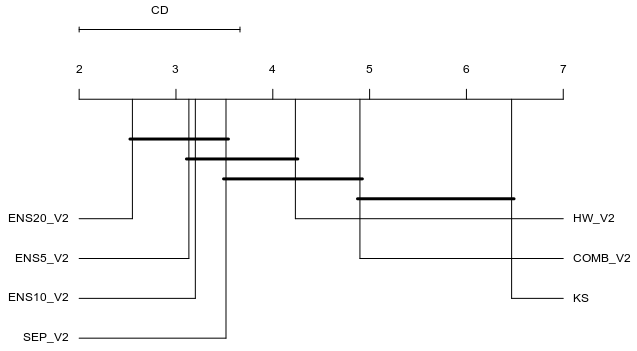
\includegraphics[scale=0.5]{images/mlp_v2_happy.png}
  \caption{Critical difference diagram for MLP using handwriting v1 for ``happy'' emotion}
  \label{fig:cd-happy}
\end{figure}

From Figure \ref{fig:cd-happy}, it can be observed that ENS20 proposed approach presented the best ranking in the Critical Difference (CD) diagram since it is located in the furthermost left position of the CD diagram. In addition, this figure shows that there is no horizontal line connecting ENS20 to any individual biometric modality, indicating a statistically significant difference between ENS20 and both individual modalities. These results only confirm the superiority, in terms of performance, of a combination approach over individual modalities, for ``happy'' emotional state. 

\begin{figure}[htbp]
  \centering
  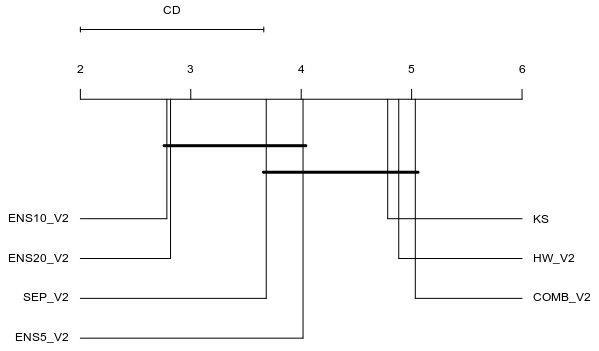
\includegraphics[scale=0.5]{images/mlp_v2_relaxed.png}
  \caption{Critical difference diagram for MLP using handwriting v1 for ``relaxed'' emotion}
  \label{fig:cd-relaxed}
\end{figure}

From Figure \ref{fig:cd-relaxed}, it can be seen that ENS10 and ENS20 proposed approaches also presented
the best rankings in the Critical Difference (CD) diagram. In addition, this figure also illustrates that there is no horizontal line connecting ENS10 and ENS20 to any individual biometric modality, indicating, once again, statistically significant differences between them and the individual modalities. Again, this result depicts that there is a superiority, in terms of performance,  of two combination approaches over individual modalities, for ``relaxed'' emotional state. 

\section{Final Remarks}

This paper presented the results of an initial investigation of how keystroke and handwriting biometrics modalities combination can impact the prediction of emotional states. In this sense, two different combination approaches (data fusion and decision fusion) were analyzed. Also, four different classification algorithms ($k$-NN, MLP, DT, and SVM) were assessed to provide a substantial amount of results to be evaluated.

After analyzing the results obtained by ``happy''  and ``relaxed'' emotional states, it is possible to state that combining keystroke and handwriting behavioral modalities generates a substantially positive impact on the emotional state prediction.
Additionally, the statistical tests proved that at least one combination approach outperforms the accuracy delivered by the individual modalities.
Having said that, the results presented in this paper bring an important contribution to the biometrics field and they can be used as a start point to new researches, especially related to combine behavioral modalities in soft biometrics prediction tasks.

As future works, we intend to explore the impact of dimensionality reduction methods in this task as well as the use of more algorithm classifiers. In the second part of the decision fusion approach, we plan to study the use of more complex and elaborated feature selection methods. Besides, the indications of a potential superiority of dynamic handwriting features will be deepen explored.
Finally, the creation of a new dataset containing more information and more biometric modalities is also listed as future work.
 
\bibliographystyle{IEEEtran}
\bibliography{IEEEfull, Referencias2}

\end{document}
